\section{Real-time Auditing Schemes}

\subsection{\small{Instant Auditing of Cloud Storage Access by Cache Partial Merkle tree}}
\begin{frame}{\normalsize{Instant Auditing of Cloud Storage Access by Cache Partial Merkle tree}}
{\tiny{2014 IEEE 6th International Conference on Cloud Computing Technology and Science}}
	\begin{center}
		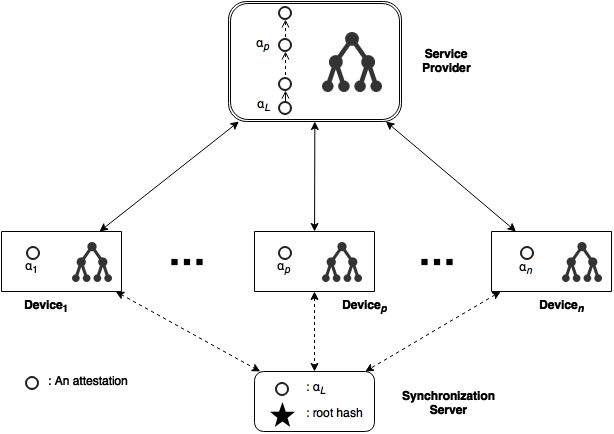
\includegraphics[width=.8\textwidth]{wei_shian}
	\end{center}
\end{frame}

\begin{frame}{Merkle Tree}
	\begin{center}
		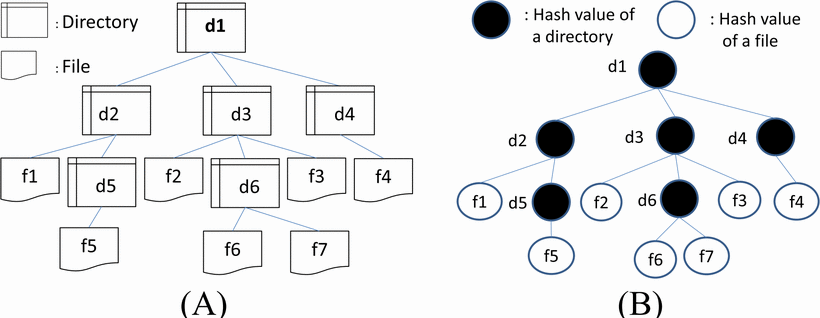
\includegraphics[width=.85\textwidth]{merkle_tree}
	\end{center}
\end{frame}

\begin{frame}{Worst-case}
	\textcolor{blue}{若有個 device 很久沒有使用,在讀寫檔案前需要更新大量未做的動作\\
	~\\
	使用者將會明顯感受到漫長的等待時間}\\
	~\\
	~\\
	~\\
	\begin{center}
		\includegraphics[width=.5\textwidth]{worst_case}
	\end{center}
\end{frame}

\subsection{\small{My Method}}
\begin{frame}{My Method}
	\textcolor{blue}{Assumption: $\text{同時有 k 個 server 上同一 file 出問題的機率} \approx 0$}
	\begin{center}
		\alert{Service Providers are Independent Cloud}
		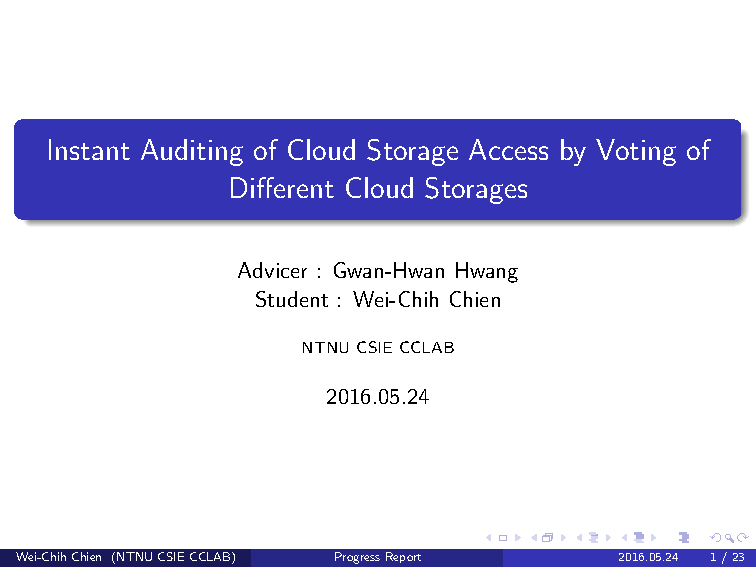
\includegraphics[width=.7\textwidth]{wei_chih}
	\end{center}
\end{frame}

\begin{frame}{Comparison}
	\begin{itemize}
		\item \textcolor{blue}{Pros}
			\begin{enumerate}
				\item Device 不用儲存、也不用修改 Merkle tree, 既省空間又省時間
				\item 資料有多份備份
				\item 解決之前的 Worst-case
			\end{enumerate}
		~\\
		\item \textcolor{red}{Cons}
			\begin{enumerate}
				\item 需要傳送多份 Request, 處理多份 Response
			\end{enumerate}
	\end{itemize}
\end{frame}